%% =============================== PREAMBLE ====================================

\documentclass[conference]{IEEEtran}

\usepackage{cite,amsmath,amssymb,amsfonts,algorithmic,graphicx,textcomp,xcolor,
etoolbox}

\pdfminorversion=7
\pdfsuppresswarningpagegroup=1
\IEEEoverridecommandlockouts
\apptocmd{\sloppy}{\hbadness 10000\relax}{}{}

\newcommand{\project}{{\sc{Collaborate}}~}
\newcommand{\cpp}{C\texttt{++}~}
\newcommand{\thisplace}{\textit{~~Dept. Elec. \& Comp. Eng.~~}\\
  \textit{The Ohio State University}\\
  Columbus, OH, USA\\
}

\title{Using Cognitive Communications to Increase the Operational Value of
  Collaborative Networks of Satellites}

\author{
  \IEEEauthorblockN{Ryan B. Linnabary}
  \IEEEauthorblockA{\thisplace linnabary.24@osu.edu}
  \and
  \IEEEauthorblockN{Andrew J. O'Brien}
  \IEEEauthorblockA{\thisplace obrien.200@osu.edu}
  \and
  \IEEEauthorblockN{Graeme E. Smith}
  \IEEEauthorblockA{\thisplace smith.8347@osu.edu}
  \and
  \IEEEauthorblockN{Christopher Ball}
  \IEEEauthorblockA{\thisplace ball.51@osu.edu}
  \and {~} \and {~~~~~~~~~~~~~~~~~~~~~~~~~~~} \and
  \IEEEauthorblockN{Joel T. Johnson}
  \IEEEauthorblockA{\thisplace johnson.1374@osu.edu}
  \and {~~~~~~~~~~~~~~~~~~~~~~~} \and {~~~~~~~~~~~~~~~~~~~~~~}
}

%% =============================== DOCUMENT ====================================

\begin{document}

\maketitle

\IEEEpubid{
  \begin{minipage}{\textwidth} {
      ~ \\ \\ \\ \\ \\ \\
      \rule{0.489\textwidth}{0.5pt} \\
      \hphantom{12pt} This research was sponsored by the NASA Advanced
      Information Sys-\\tems Technology Program NNH16ZDA001N-AIST. \\ \\
      \normalsize
      978-1-7281-0048-7/19/\$31.00 \copyright2019 IEEE
    }
  \end{minipage}
}

%% =============================== ABSTRACT ====================================

\begin{abstract}

  Distributed satellite constellations utilizing networks of small satellites
will be a key enabler of new observing strategies in the next generation of NASA
missions.  While it is quickly becoming feasible to establish communication
networks among small satellites, a critical question is how these networks can
be best utilized to achieve objectives.  Small satellite instruments are
becoming more capable, but they are still resource constrained (i.e. power,
data, scanning systems, etc.).  Adaptive instruments that intelligently adjust
parameters {\color{black} on the fly} are essential for increasing operational
value within these constraints, and the primary purpose of collaborative
communication among small satellites is to achieve system-level adaptivity.
This could dramatically increase the complexity of the control algorithms for
small satellite communication networks.  Application of cognitive communication
is one promising method to address this problem.  In this paper, we discuss our
recent investigations into how machine learning (ML) algorithms can be utilized
in the high-level decision making of a communication system in a distributed
satellite mission.

\end{abstract}

\vspace{8pt}

\begin{IEEEkeywords}

  Distributed Satellite Missions, Autonomous Systems, Sensor Network, Sensor
Web, OSSE

\end{IEEEkeywords}

%% ============================= INTRODUCTION ==================================

\section{Introduction}
\label{sec:intro}

It is envisioned that NASA's future space systems will be composed of large,
inhomogeneous networks of small satellites and autonomous platforms \cite{ref1}.
These resource constrained systems, carrying an array of different instruments,
will be expected to operate autonomously and collaboratively to achieve mission
and science goals.  Unfortunately, current and near-future inter-satellite
communications are highly constrained in terms of link availability,
reliability, power and bandwidth.  Although future technologies (such as free
space optical links) may alleviate some constraints, it is expected that future
instruments will rapidly expand in both data volume and sensor reconfigurability
\cite{ref2}.  In this way, it is not sufficient to simply increase the
capabilities of the communication links.  Rather, it is also necessary to
improve the complex decision making that communication systems perform, such as
deciding when to transmit, what information is valuable to nodes of the network,
and how to adapt local operations following the reception of new information.
Recently, cognitive space communication algorithms have been proposed as a
solution to address the complexity of future inter-satellite communication
systems \cite{ref3}.

In this work, we show results of simulation studies to explore the advantages
that cognition could offer for collaborative small-satellite networks.  Under a
NASA Advanced Information System Technology program, we are currently developing
an open-source \cpp library for the simulation of autonomous and collaborative
networks of adaptive sensors \cite{ref6}.  This library and accompanying
utilities allow for the efficient simulation of networks of satellites with
realistic constraints in communication, power, and measurements.  A key focus of
this software is the simulation of sensors that operate adaptively.  Adaptive
sensors must make intelligent decisions regarding their configuration based on
their own measurements as well as the measurements provided by other sensors in
a network.  However, the extreme complexity of the decision space makes the
development of optimal decision-making systems very difficult.  Thus, an
approach based on cognition could offer an appealing solution.  We investigate
how our simulation tools could be useful for production of large training
data-sets that capture the operation of collaborative, adaptive networks of
small satellites.  We then investigate how such a data-set could be combined
with machine learning techniques to train neural networks that could make
intelligent decisions about when and what to communicate.  The applicability of
these methods to future cognitive space communication will be discussed.

%% ========================= HIGH-LEVEL COGNITION ==============================

\section{Identifying a Role for Cognition in High-Level Communications} \label{sec:hlc}

\textit{Cognition} refers to the act of selecting and carrying out actions based
on both specific {\color{black} goals and perception of an external
environment}.  Key to cognition is the perception-action cycle depicted in
Figure \ref{fig:figure1}.  Cognition necessarily includes learning from past
experiences and {\color{black} interactions with the environment}.  Thus, a
\textit{cognitive entity} is capable of taking action based on its
{\color{black} goals and perception of the environment}, potentially learning
from the result of its action.  It is an intelligent entity that possesses
perception, learning, reasoning, and making decisions
\cite{ref7}. \textit{Cognitive Communications} are communications whose
operations are in some way dependent on cognition.

\begin{figure}[t!]
  \begin{center}
    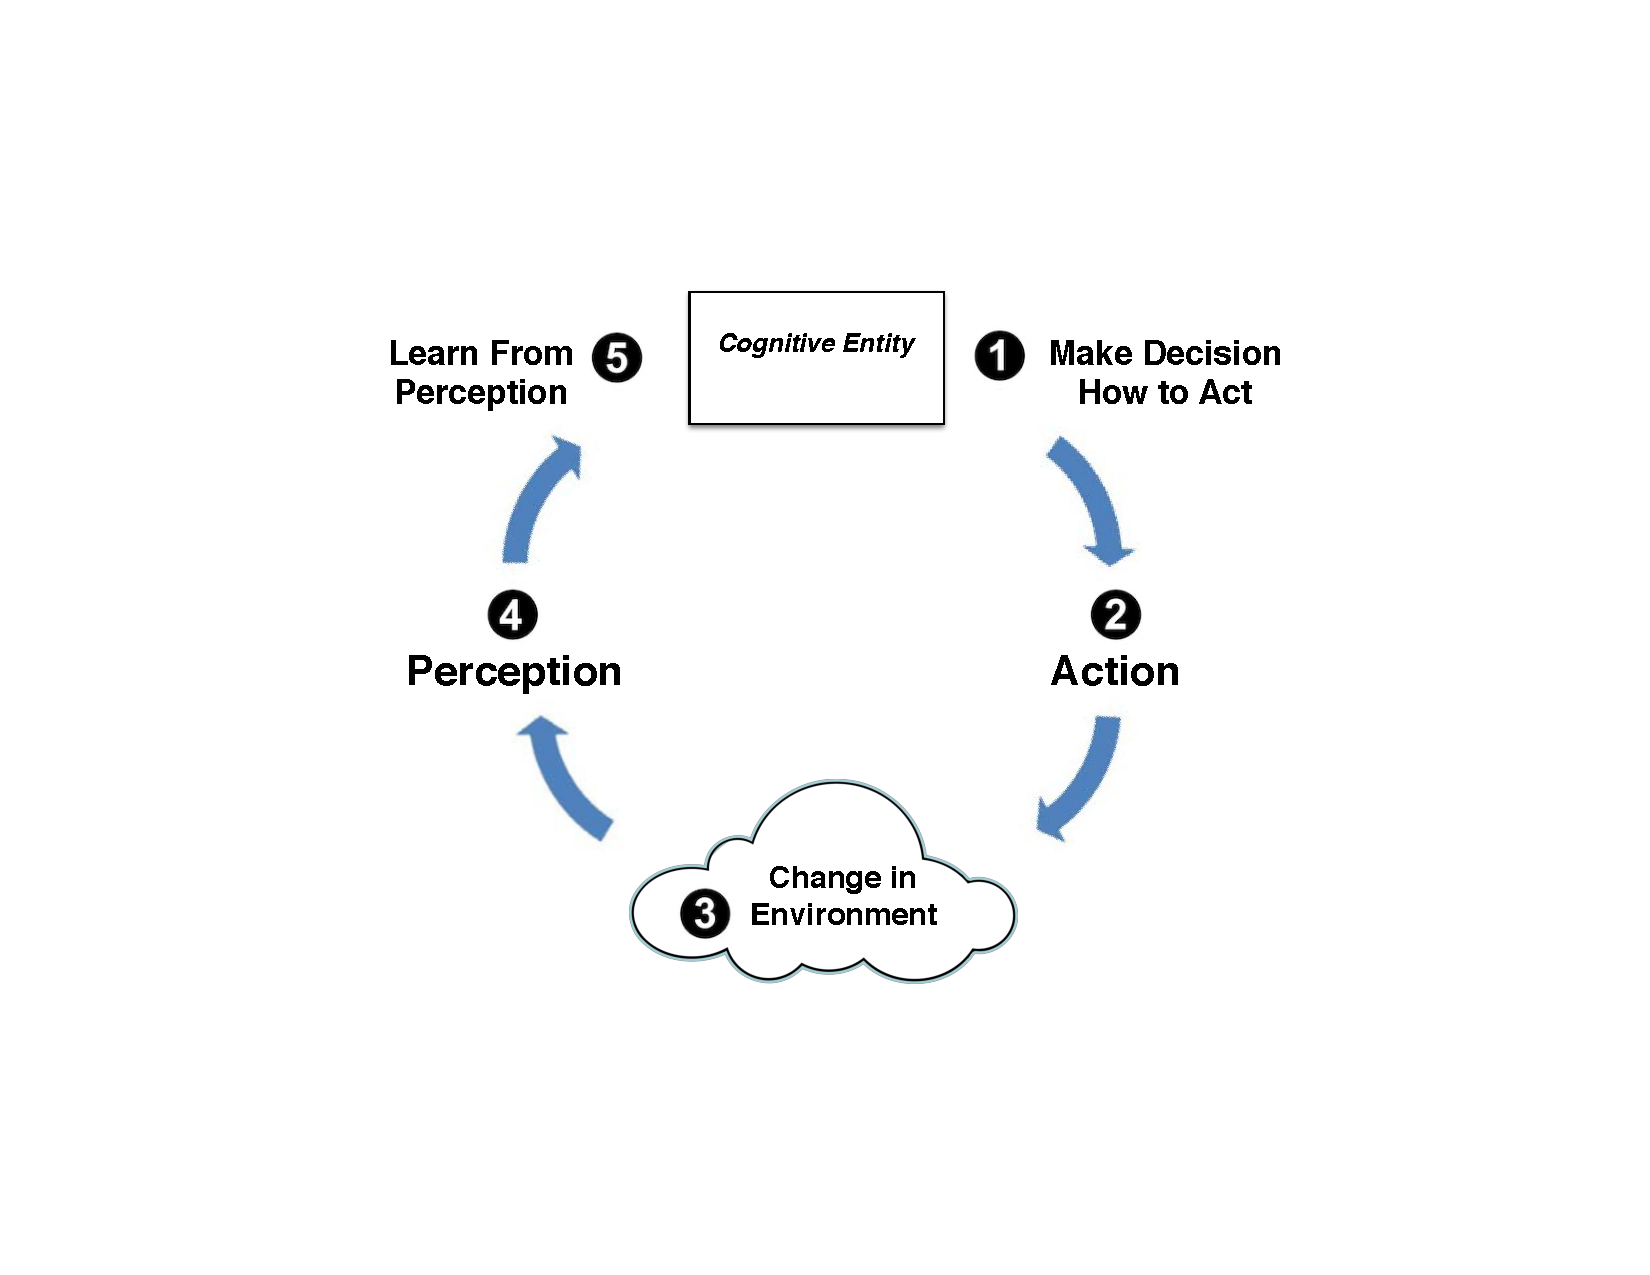
\includegraphics[width=0.8\linewidth] {images/Figure1.pdf} \\
  \end{center}
  \caption{Fundamental process of cognition, the perception-action cycle.}
  \label{fig:figure1}
\end{figure}

Research into cognitive communication algorithms for satellite systems have
focused on communications at a low level, including decision making regarding
modulation, power, bandwidth, and error rate.  For example, on-line machine
learning was used to optimize the selection of of software-defined radio
parameters in \cite{ref4}.  Cognitive digital beamforming has also been applied
to satellite communication \cite{ref5}.  However, cognition can also be applied
to the higher-level aspects of a communication system, such as the intelligent
routing of information within an autonomous satellite sensor network
\cite{ref7}.

Cognition may also offer an improvement in the complex, higher level decisions
of communication in the context of mission and science objectives.  At this
level, cognition is applied to the operation of the network with the decision
making primarily influenced by the constraints of the space communication
network links.  Communication networks within distributed small satellite
constellations will enable collaborative operations, and, when these satellites
are equipped with adaptive sensors, collaborative communications will enable
system-level adaptivity.

In order to illustrate this, consider an example sequence of events shown in
Figure~\ref{fig:figureColab}.  In this scenario, Satellite ``A'' measures
cloud depth in the Pacific Ocean (blue line).  It then predicts the arrival of a
follow-up satellite and relays a message through satellites ``B'' and ``C'' to
queue ``D'' for a measurement with a different sensor (red line).  After the
second measurement is made, information is fed back to the originating satellite
(Satellite ``A''), so it can learn about how valuable the information was and
how successful the communication route over the network was.

\begin{figure}[b!]
  \begin{center}
    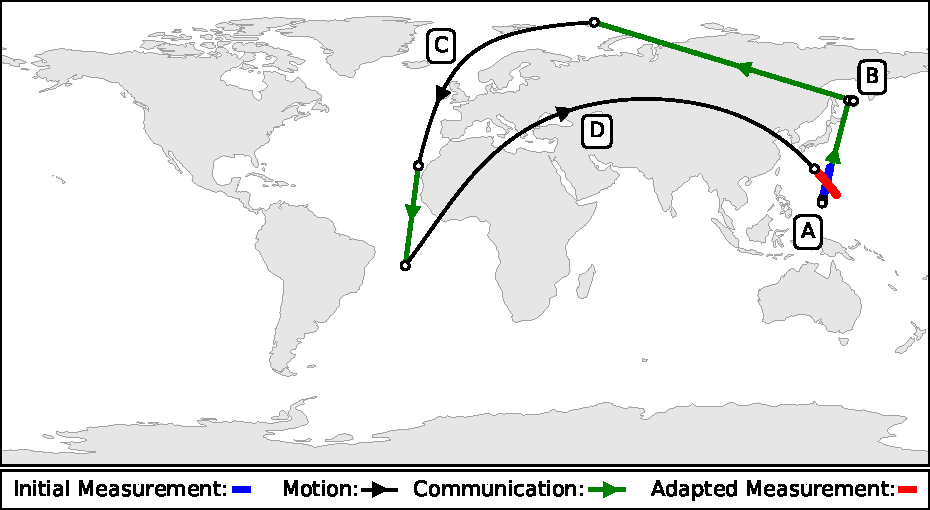
\includegraphics[width=0.9\linewidth] {images/collaborate.pdf} \\
  \end{center}
  \caption{Example sequence of collaboration between satellites in a constellation.}
  \label{fig:figureColab}
\end{figure}

Figure~\ref{fig:figure2} shows a depiction of the perception-action cycle as it
applies to our scenario of interest.  Here, a small satellite serves as the
cognitive entity.  The action it takes is to determine what information to send
and what route to try to send it on.  This action influences the rest of the
small satellite constellation by causing them to adjust their sensors and make
measurements in an improved manner.  The information about this influence is fed
back to the original satellite so that it can learn from this reaction.

\begin{figure}[b!]
  \begin{center}
    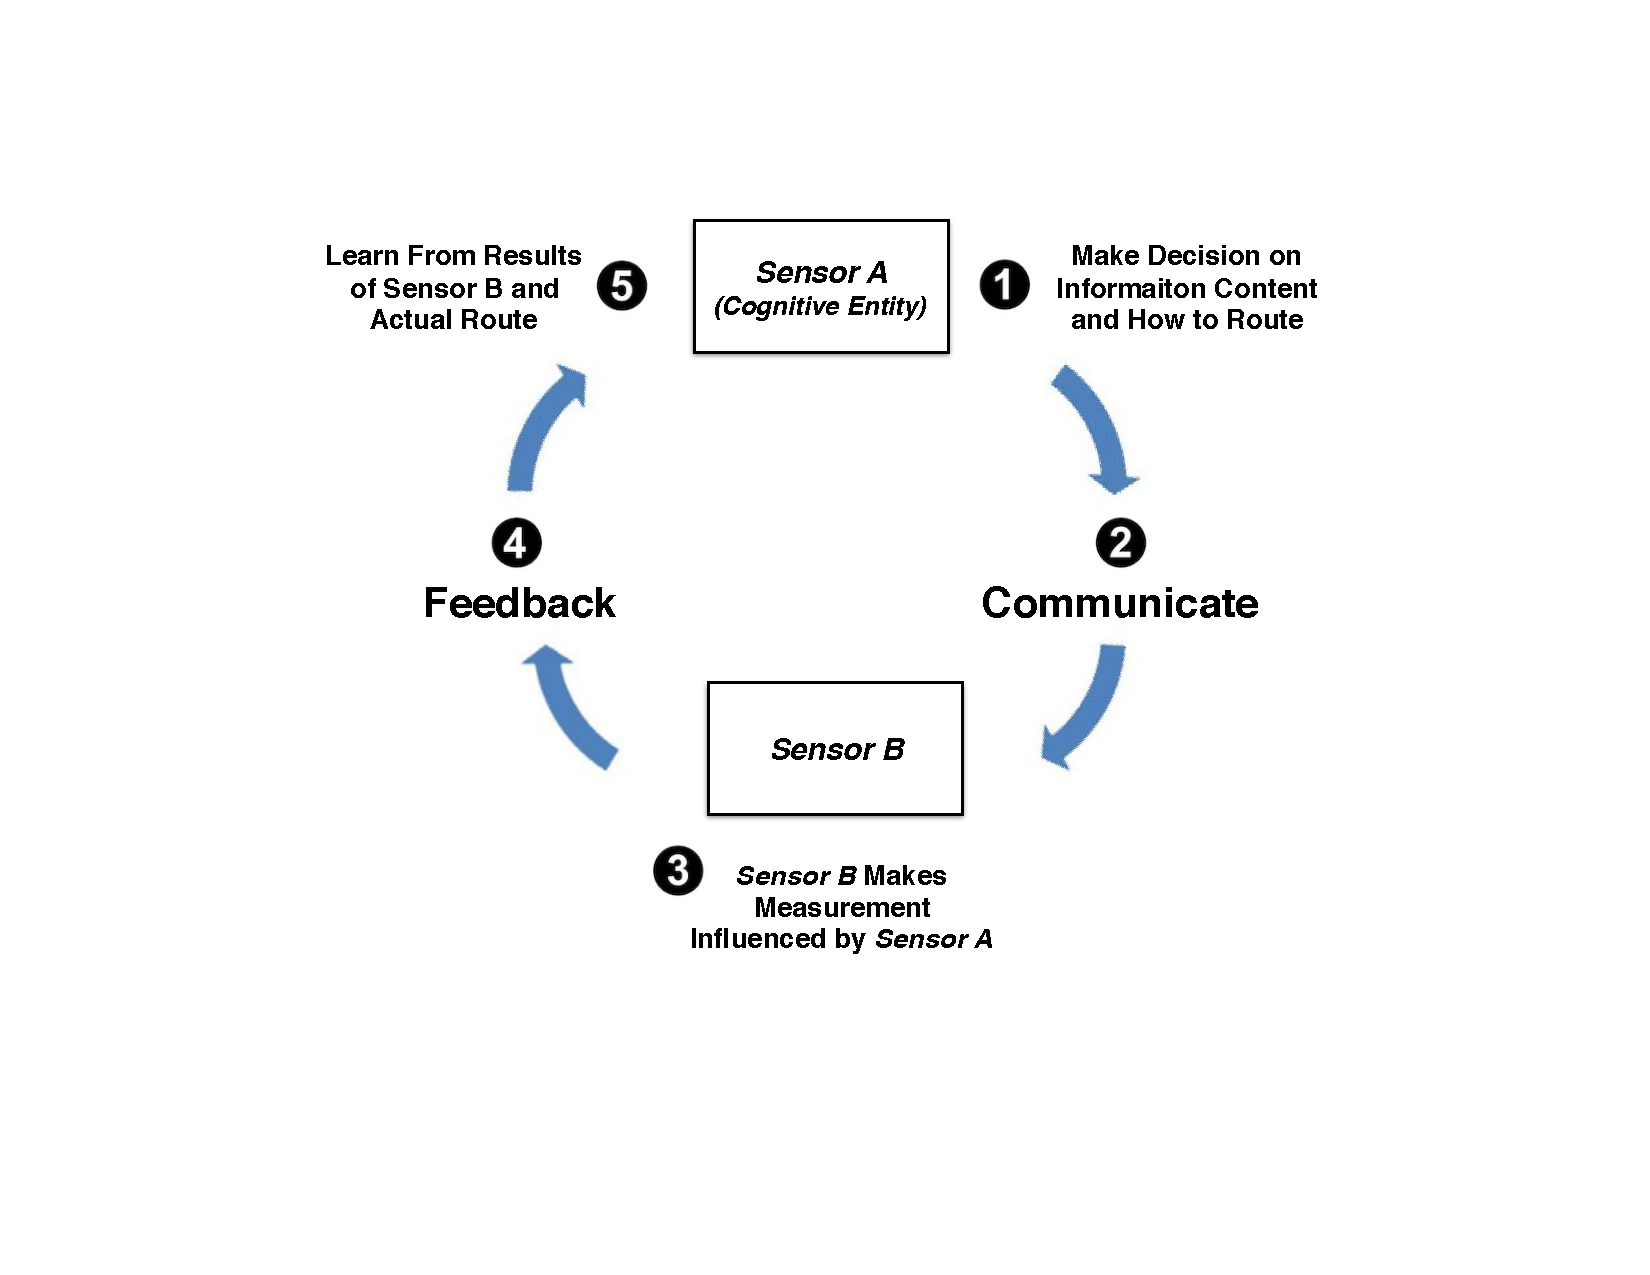
\includegraphics[width=0.9\linewidth] {images/Figure2.pdf} \\
  \end{center}
  \caption{Perception-action cycle of cognition as applied to collaborative communications between satellites.}
  \label{fig:figure2}
\end{figure}

The problem that prevents a practical implementation of the model shown in
Figure \ref{fig:figure2} is that the decision-making and learning processes is
very difficult to model and design.  This is especially true when considering
the significant uncertainty at any given moment given the state of the
constellation and the communication routes available.  Machine Learning (ML) is
one approach to overcome this problem.  Machine learning techniques are
currently being applied in the development of adaptive hardware, resource
optimization, and other areas of sensor network design.  An opportunity exists
here to use machine learning to optimize information flow within a collaborative
network of satellites.  Improvements would increase communications efficiency by
increasing the value of data contents and reducing operational resource
consumption.

The most common machine learning categories (i.e. regression and classification)
can be applied to high-level network management tasks.  Regression tasks enable
satellites to autonomously adjust parameters for communication, sensing, and
on-board data processing.  Classification of network nodes based on proximity
and capabilities could increase efficiency by informing antenna direction or
temporal scheduling.  %Our research is exploring this new application using
existing machine learning algorithms, a key part of which is the generation of
training data.

\section{Sensor Network Simulations to Support Machine Learning}
\label{sec:software}

%% =============================== SOFTWARE ====================================

A software tool-set \project is under development which is capable of producing
the training data for ML algorithms.  The tool-set has two main components:
first, a \cpp development library for observing system simulation experiments;
and second, a Python visualization and analysis package for post-processing of
data.  The project is published to a Git repository under the GPLv3.0 license.

\begin{figure}[t!]
  \begin{minipage}[b]{\linewidth}
    \begin{center}
      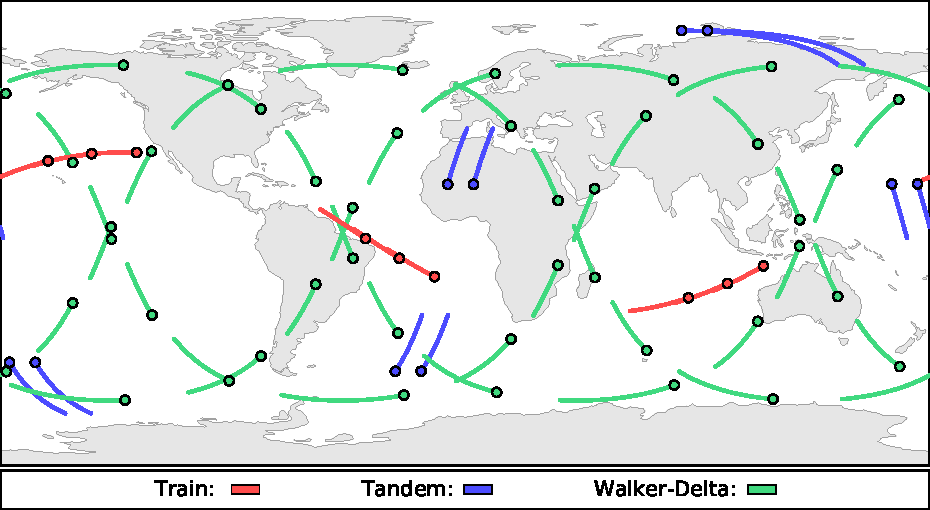
\includegraphics[width=0.9\textwidth]{images/constellations.pdf} \\
      {\footnotesize(a) Various constellations defined by orbit patterns}
    \end{center}
    \medskip
  \end{minipage}
  \begin{minipage}[b]{\linewidth}
    \begin{center}
      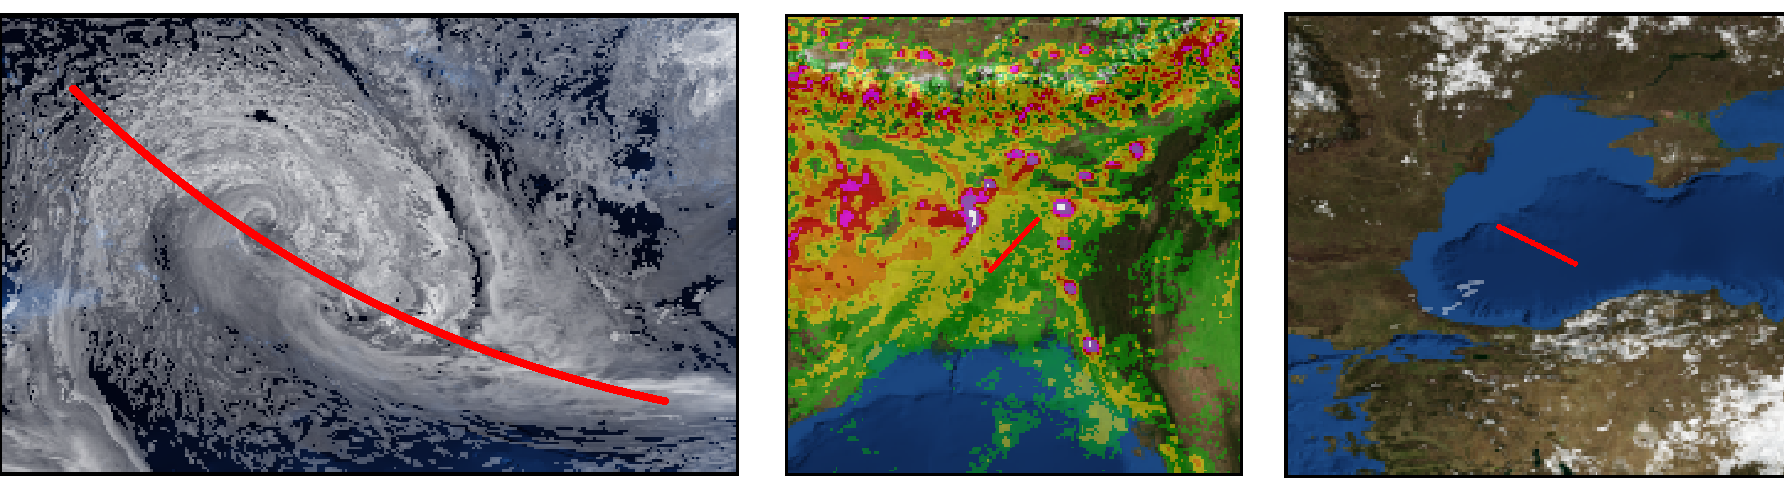
\includegraphics[width=0.9\textwidth]{images/remote_sensing.pdf} \\
      {\footnotesize{
          \color{white}~~~~~~\color{black}
          (b) Cloud Depth~~~~~~~~~~
          (c) Precipitation~~~~
          (d) Optical Images}}
    \end{center}
    \medskip
  \end{minipage}
  \begin{minipage}[b]{\linewidth}
    \begin{center}
      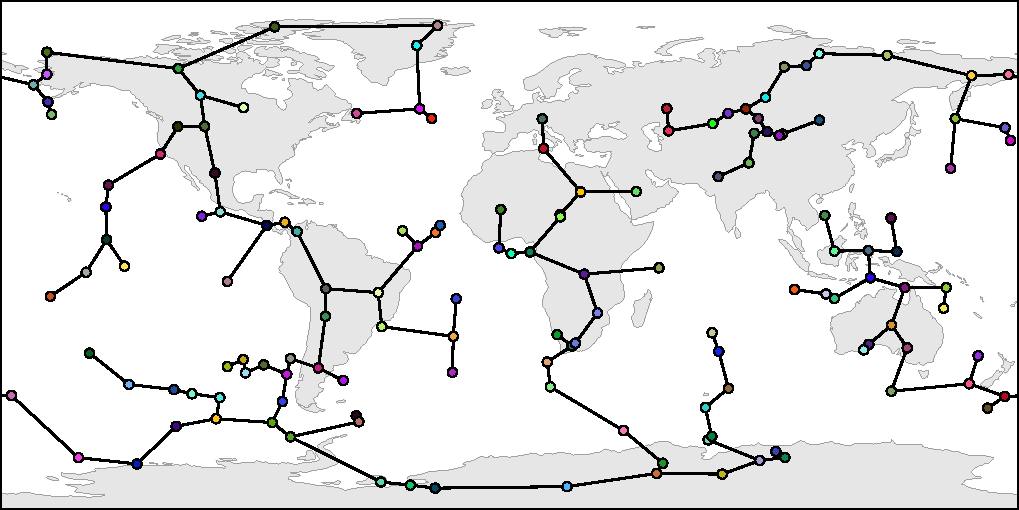
\includegraphics[width=0.9\textwidth]{images/prim.pdf} \\
      {\footnotesize(e) Instantaneous network graph structure (minimum spanning
        tree)}
    \end{center}
  \end{minipage}
  \caption{\project software features}
  \label{fig:features}
\end{figure}

The \project library offers a number of unique features valuable to future
observing system simulation experiments.  At its core, it is a physics engine
for satellite position, velocity, and attitude.  Power and RF accessories may be
attached to satellites and individually oriented.  The next level involves rapid
constellation design.  Standard orbit models described by two-line-element (TLE)
sets are provided, copied, and modified to generate novel and interesting
constellation patterns.  Examples are illustrated in
Figure~\ref{fig:features}(a).  Sensor hardware is attached to satellites as an
interface to truth data (NetCDF Nature Run data).  This provides a custom
modeling environment for real sensor hardware and enables heterogeneous sensor
constellations with different capabilities.  As a satellite orbits, its pointing
vector intersects Earth's surface or an atmospheric layer and samples the
underlying data, as shown in Figure~\ref{fig:features}(b-d).

\project is named for its ability to manage collaborative networks of
satellites.  Its implementation focuses on the high-level communication decision
space discussed previously.  The library employs, in addition to standard \cpp
components, advanced data structures including trees and graphs to execute
predictive route-finding algorithms for efficient communications.  For example,
line-of-sight wireless channels are captured in a graph, as illustrated in
Figure~\ref{fig:features}(e), the minimum spanning tree.

The software logs simulation data to files accessible by external machine
learning tools.  \project was developed around simple data formats for
portability and to promote development of custom analysis tools.  Primarily,
data is serialized and written to binary files.  These formats are well
documented and easy to parse in Python or other scripting languages.  Included
Python packages understand the data formats and can read and store the data for
later use as Numpy or Pandas data structures.  Examples include time-series data
frames or network adjacency matrices (weighted and unweighted).
Figure~\ref{fig:data} shows several common data structures in memory; one to
store satellite parameters; and another for network structures.

\begin{figure}[b]
  \begin{minipage}[b]{0.49\linewidth}
    \begin{center}
      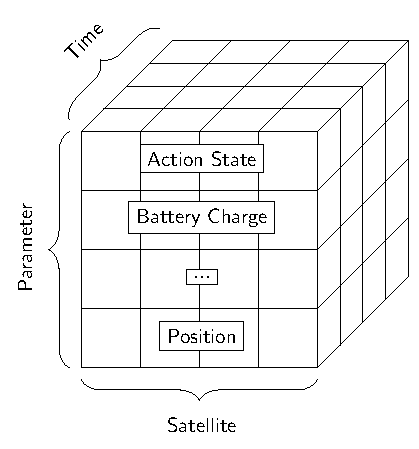
\includegraphics[width=0.86\textwidth]{images/params.pdf} \\
      {\footnotesize(a) Satellite parameter data}
    \end{center}
  \end{minipage}
  \begin{minipage}[b]{0.49\linewidth}
    \begin{center}
      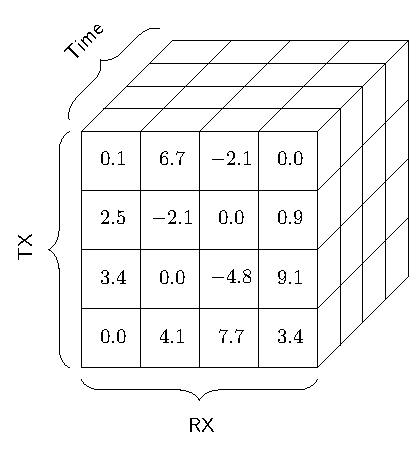
\includegraphics[width=0.86\textwidth]{images/weighted.pdf} \\
      {\footnotesize(b) Network parameter data}
    \end{center}
  \end{minipage}
  \caption{Simulation training data formats}
  \label{fig:data}
\end{figure}

Python scripts are provided not only for receiving simulation data at a low
level, but also many high level analysis tasks.  In fact, all figures in this
document were produced using the tools provided by the library.  Primary
third-party packages used include the following: Numpy, Pandas, Cython, NetCDF4,
Matplotlib, Cartopy, Scikitlearn, TensorFlow, and SciPy.  These enable post
processing for plots and animations or to train machine learning algorithms.
Numpy and Pandas provide powerful linear algebra and statistics operations.
Cartopy provides extensive map projections and transformations which support
visualizing satellite positions and truth data.  Machine learning algorithms are
available in the Scikitlearn and Tensorflow packages, which interface well with
Numpy and Pandas structures.  For example, satellite parameter data
(Figure~\ref{fig:data}(a)) is plotted in Figure~6. %to expose and potentially
exploit correlations.  Several of these seem strongly correlated and many are
also periodic.  Potential high-level communications optimizations may involve
predicting when a satellite has the most visible neighbors (available
line-of-sight links).  An algorithm for power management scheduling may use the
instantaneous charge or power to plan efficient sensor operation.

\begin{figure}[t]
  \begin{center}
    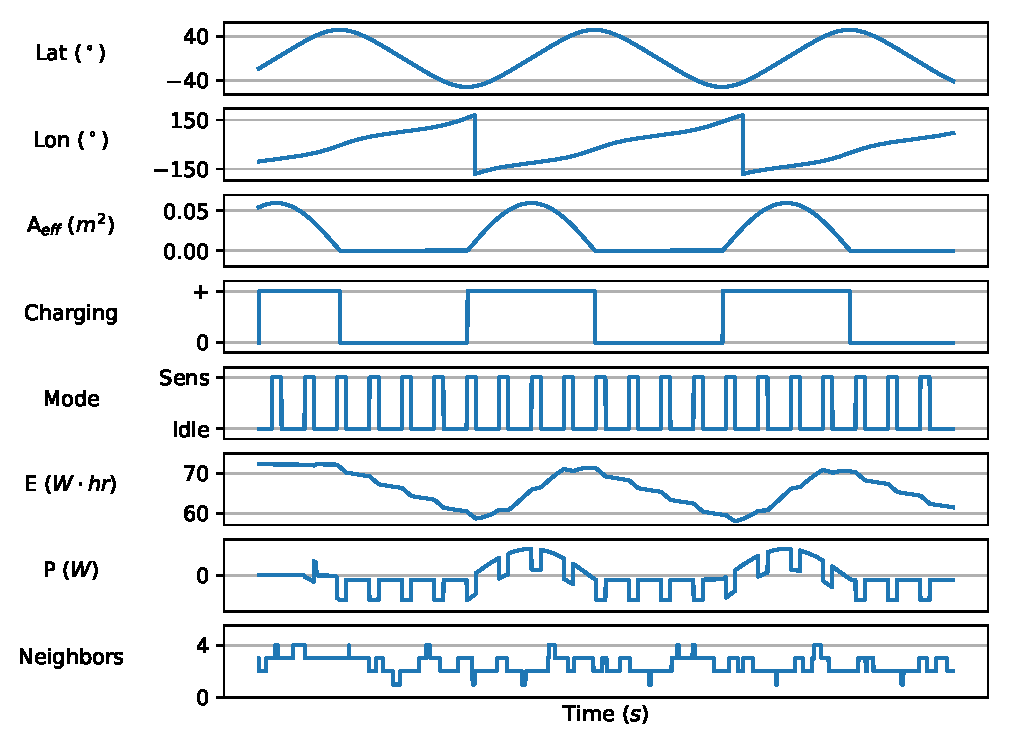
\includegraphics[width=0.9\linewidth]{images/param_plot.pdf}
  \caption{Example parameters versus time from simulation data}
  \end{center}
  \label{fig:processing}
\end{figure}

%% =============================== EXAMPLES ====================================

\section{Example Case Studies}
\label{sec:examples}

The following examples demonstrate cognitive communications and machine learning
techniques applied to software simulations.  First, parametric regression is
automated using the \project network feedback algorithm.  This simulates
deployed machine learning in a realistic observing system.  Second, satellites
are classified based on line-of-sight proximity.  This demonstrates the utility
of \project simulation data for training external machine learning models.

\subsection{Cognitive Feedback For Autonomous Parameter Regression}
\label{ssec:feedback}

\begin{figure}[b!]
  \begin{minipage}[b]{\linewidth}
    \begin{center}
      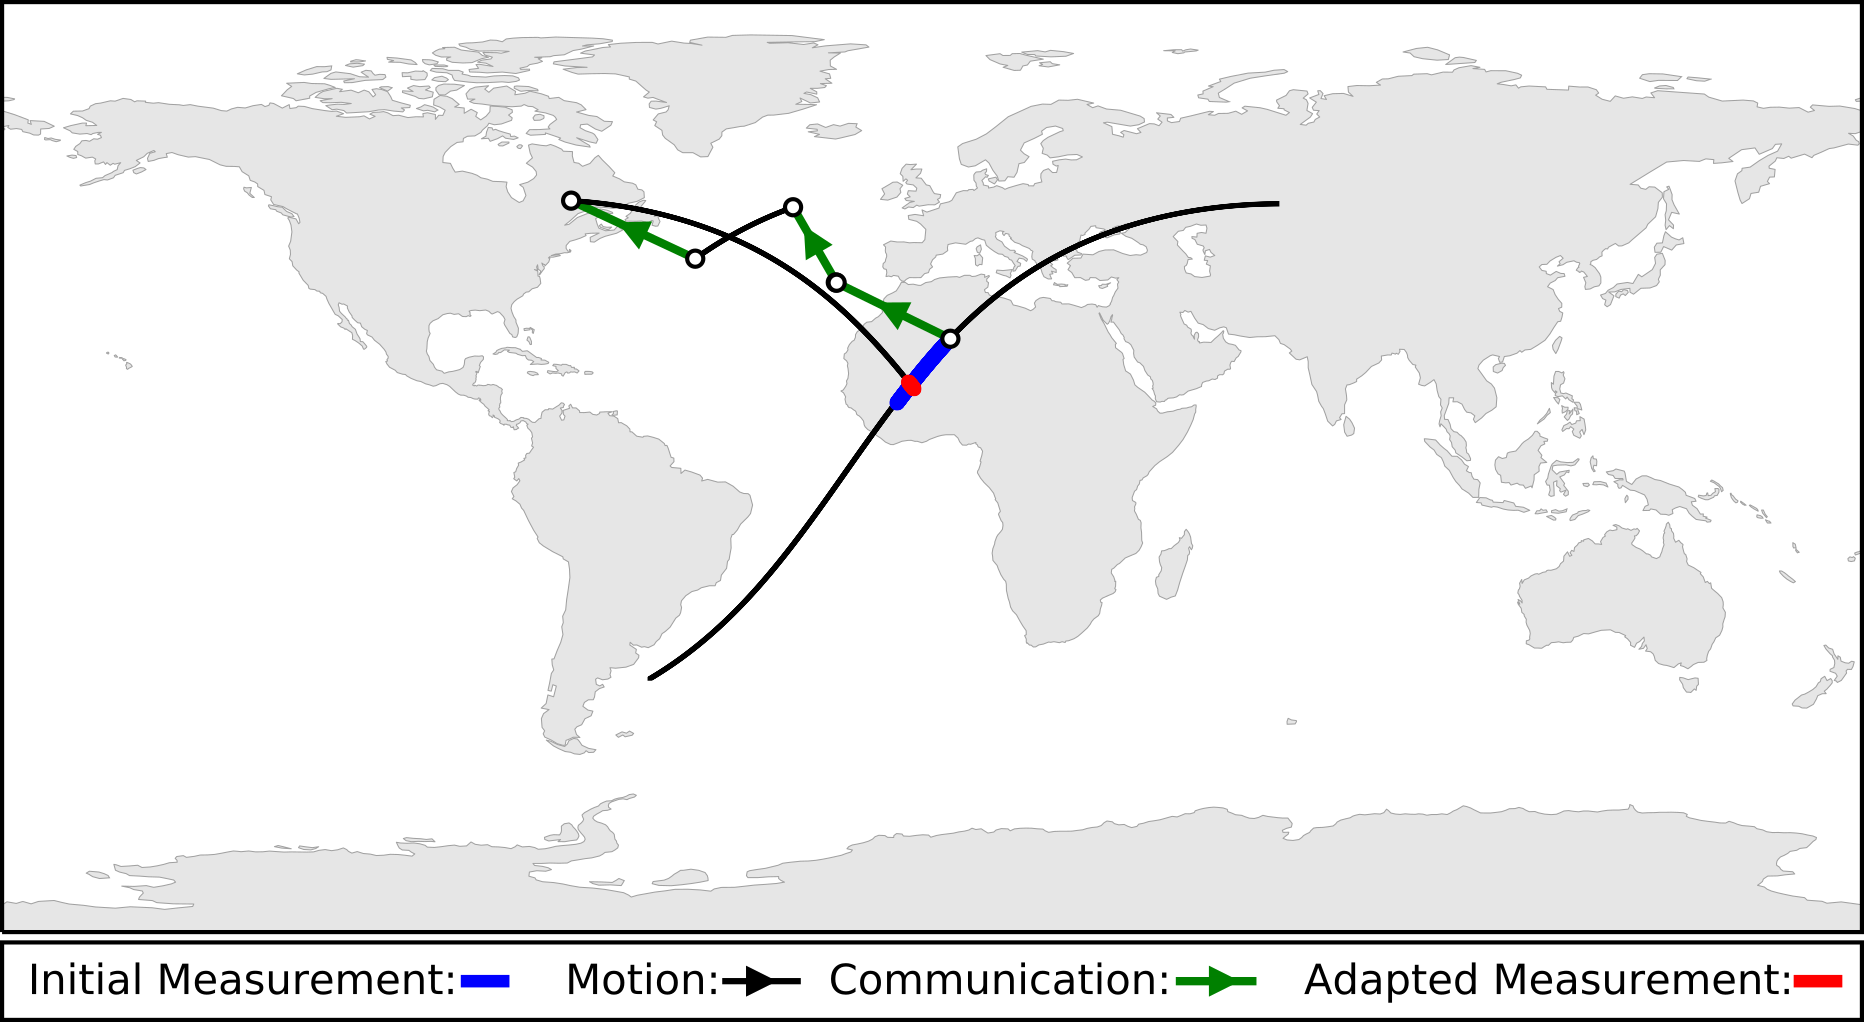
\includegraphics[width=0.9\textwidth]{images/half_loop.png} \\
      {\footnotesize(a) Forward route}
    \end{center}
  \end{minipage}
  \begin{minipage}[b]{\linewidth}
    \begin{center}
      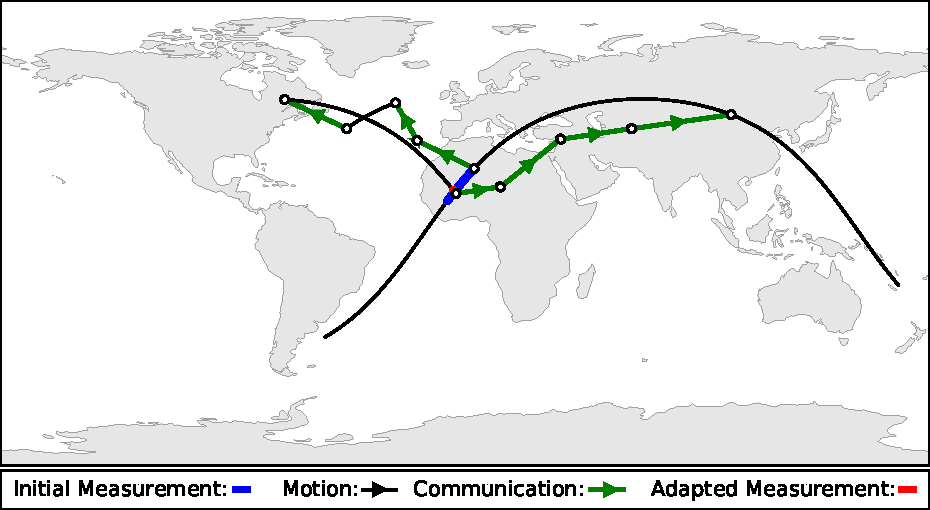
\includegraphics[width=0.9\textwidth]{images/loop.pdf} \\
      {\footnotesize(b) Feedback route}
    \end{center}
  \end{minipage}
  \begin{minipage}[b]{\linewidth}
    \begin{center}
      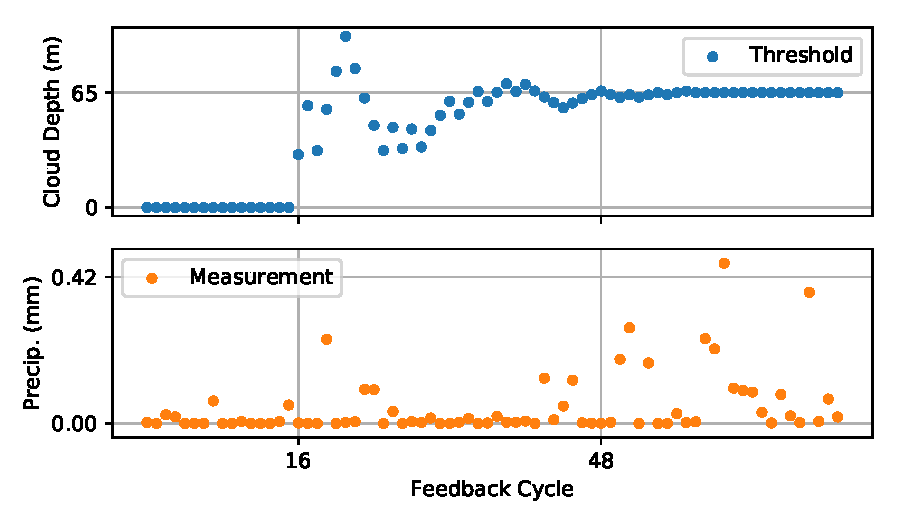
\includegraphics[width=0.9\textwidth]{images/regression.pdf} \\
      {\footnotesize(c) Autonomous parametric regression for data correlation
        threshold}
    \end{center}
  \end{minipage}
  \caption{Cognitive communications feedback}
  \label{fig:feedback}
\end{figure}

Section~\ref{sec:software} shows that \project provides a network algorithm for
predicting optimal routes, such as the one illustrated in
Figure~\ref{fig:figureColab}; this can also be used to predict a path for
feedback to the original satellite.  A single feedback cycle is shown in
Figure~\ref{fig:feedback}(a-b).  In this plot, a cognitive satellite travels
from South America over the Atlantic and senses data over Africa (blue line).
Internal processing reveals that the science value of a follow-up measurement
exceeds expected resource costs, so the satellite predicts the arrival of
another sensor platform.  A message is forwarded through the network over the
Pacific to queue the next measurement.  After a follow-up measurement, data is
fed back to the original satellite over the Middle East and China.  The contents
of this feedback message inform corrective action by the cognitive satellite.

Science value optimization is demonstrated by a 24-hour simulation where this
feedback cycle is repeated 75 times.  In this simulation, the cognitive
satellite performs a regression task to discover the correlation between cloud
depth and precipitation.  The top plot in Figure~\ref{fig:feedback}(c)
illustrates regression of the target parameter (cloud depth threshold for
non-zero precipitation).  Initially the threshold is set to 0 meters and the
cloud radar requests follow-up precipitation measurements indiscriminately.  For
the first 16 regression cycles in the bottom plot of
Figure~\ref{fig:feedback}(d), 20 percent of the precipitation sensors measured
non-zero precipitation.  At 16 cycles the satellite begins adjusting the
threshold, which converges to a value of 65 meters after 32 cycles.  The new
threshold improves operational science return by increasing the number of
non-zero precipitation measurements to 50 percent.

\subsection{Spectral Clustering Using Simulated Network Data}
\label{ssec:cluster}

Simulation data described in Figure~\ref{fig:data}(b) is produced by a
simulation and used to train a machine learning (classification) algorithm.  The
data contains a time series of adjacency matrices with edge weights equal to
line-of-sight distances between nodes.  A single frame of this data is inverted
and normalized to produce an affinity matrix suitable for ScikitLearn's
SpectralClustering algorithm.  This algorithm identifies normalized cuts in the
graph and separates nodes into groups.  Figure~\ref{fig:clusters}(a-c) show how
a graph is sorted and reduced to isolate groups of nodes based on proximity.
Figure~\ref{fig:clusters}(d) shows the 15 clusters using actual satellite
positions.

\begin{figure}[t!]
  \begin{minipage}[b]{0.32\linewidth}
    \begin{center}
      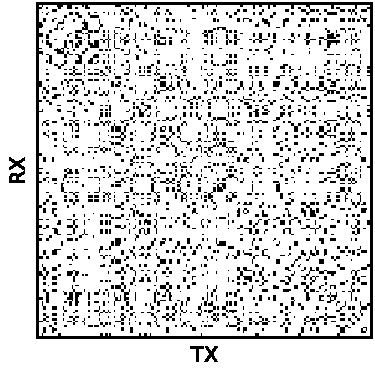
\includegraphics[width=\textwidth]{images/los_matrix.pdf} \\
      {\footnotesize(a) LOS Matrix}
    \end{center}
  \end{minipage}
  \begin{minipage}[b]{0.32\linewidth}
    \begin{center}
      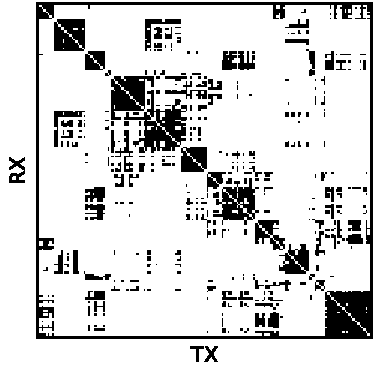
\includegraphics[width=\textwidth]{images/sorted_matrix.pdf} \\
      {\footnotesize(b) Sorted Clusters}
    \end{center}
  \end{minipage}
  \begin{minipage}[b]{0.32\linewidth}
    \begin{center}
      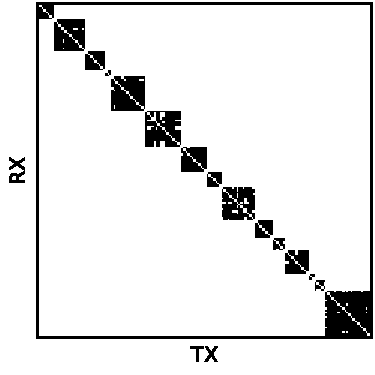
\includegraphics[width=\textwidth]{images/cluster_matrix.pdf} \\
      {\footnotesize(c) Isolated Clusters}
    \end{center}
  \end{minipage}
  \begin{minipage}[b]{\linewidth}
    \medskip
    \begin{center}
      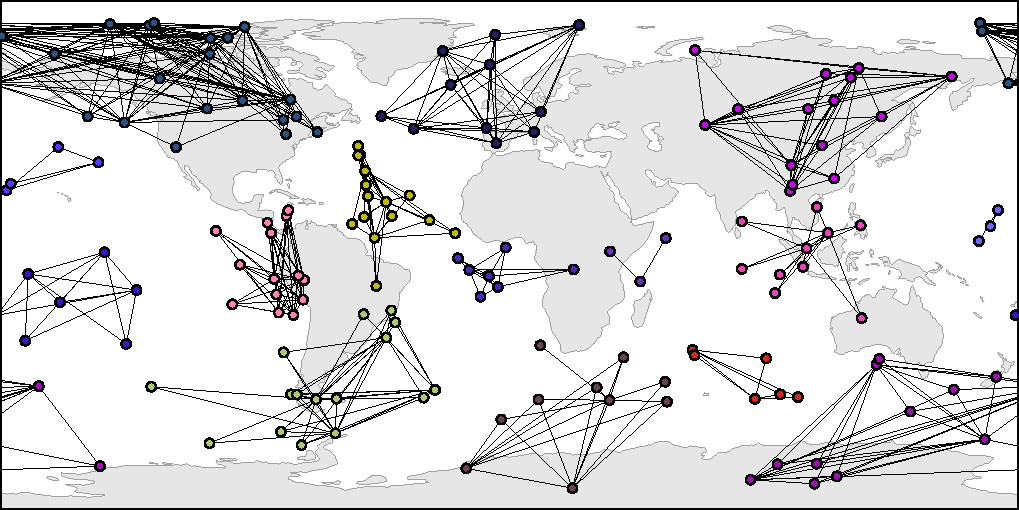
\includegraphics[width=\textwidth]{images/clusters.pdf} \\
      {\footnotesize(d) Map of isolated clusters}
    \end{center}
  \end{minipage}
  \caption{Spectral clustering by k-means classification}
  \label{fig:clusters}
\end{figure}

\vfill
\break

\project currently supports one-to-one communication, but future network schemes
will require one-to-many links and will likely employ clustering as a single
part of its optimization routine.  For example a satellite may strategically
orient its antenna toward the center of its cluster, maximizing signal strength
for its immediate neighbors.

%% =============================== REFERENCES ==================================

\small
\begin{thebibliography}{9}
\bibitem{ref1} {
    Gilbert J. Clark, Wesley Eddy, Sandra K. Johnson, David E. Brooks, and
    James L. Barnes, ``Architecture for Cognitive Networking within NASA’s
    Future Space Communications Infrastructure'', 34th AIAA International
    Communications Satellite Systems Conference. Cleveland, OH.}
\bibitem{ref2} {
    A. G. Schmidt, G. Weisz, M. French, T. Flatley and C. Y. Villalpando,
    ``SpaceCubeX: A Framework For Evaluating Hybrid Multi-Core CPU/FPGA/DSP
    Architectures,'', \textit{IEEE Aerospace Conference}, Big Sky, MT, 2017,
    pp. 1-10.}
\bibitem{ref3} {
    J. Barnes and W. Eddy, ``Machine learning for space communications service
    management tasks'' 2017 Cognitive Communications for Aerospace Applications
    Workshop (CCAA), Cleveland, OH, 2017, pp. 1-4.
  }
\bibitem{ref4} {
    P. V. R. Ferreira et al.,
    ``Multi-objective reinforcement learning-based deep neural networks for
    cognitive space communications''
    2017 Cognitive Communications for Aerospace Applications Workshop (CCAA),
    Cleveland, OH, 2017, pp. 1-8.
  }
\bibitem{ref5} {
    Wenhao Xiong, J. Lu, X. Tian, G. Chen, K. Pham and E. Blasch, ``Cognitive
    radio testbed for Digital Beamforming of satellite communication'' 2017
    Cognitive Communications for Aerospace Applications Workshop (CCAA),
    Cleveland, OH, 2017, pp. 1-5.
}
\bibitem{ref6} {
    R. B. Linnabary, A. O'Brien, G. E. Smith, C. D. Ball, and J. T. Johnson,
    ``Open Source Software For Simulating Collaborative Networks Of Autonomous
    Adaptive Sensors'', submitted to {\it Proceedings of the IEEE International
      Geoscience and Remote Sensing Symposium}, January 2019.}
\bibitem{ref7} {
    G. E. Smith, A. E. Mitchell, C. D. Ball, A. O'Brien, and J. T. Johnson,
    ``Fully adaptive remote sensing observing system simulation experiments'',
    in {
      \it Proceedings of the IEEE International Geoscience and Remote Sensing
      Symposium} , July 2018, pp. 5839-5842.}
\end{thebibliography}

\end{document}
